\documentclass[journal]{IEEEtran}

% *** GRAPHICS RELATED PACKAGES ***
%
\ifCLASSINFOpdf
  \usepackage{graphicx}
  \graphicspath{ {./images/} }
  \usepackage{amsmath}
  \DeclareMathOperator*{\argmax}{arg\,max}
  \DeclareMathOperator*{\argmin}{arg\,min}
  \usepackage{caption}
  \usepackage{subcaption}
  \usepackage{hyperref}
  \usepackage[sorting=none]{biblatex}
  \addbibresource{biblio.bib}
\else
\fi

% correct bad hyphenation here
\hyphenation{op-tical net-works semi-conduc-tor}


\begin{document}
%
% paper title
% Titles are generally capitalized except for words such as a, an, and, as,
% at, but, by, for, in, nor, of, on, or, the, to and up, which are usually
% not capitalized unless they are the first or last word of the title.
% Linebreaks \\ can be used within to get better formatting as desired.
% Do not put math or special symbols in the title.
\title{DeepProbLog Tasks}
%
%
% author names and IEEE memberships
% note positions of commas and nonbreaking spaces ( ~ ) LaTeX will not break
% a structure at a ~ so this keeps an author's name from being broken across
% two lines.
% use \thanks{} to gain access to the first footnote area
% a separate \thanks must be used for each paragraph as LaTeX2e's \thanks
% was not built to handle multiple paragraphs
%

\author{Davide~Lusuardi,~223821,~\IEEEmembership{davide.lusuardi@studenti.unitn.it}% <-this % stops a space
}

% The paper headers
% \markboth{BIO-INSPIRED ARTIFICIAL INTELLIGENCE, UNITN, JULY~2022}%
% {}

% make the title area
\maketitle

% As a general rule, do not put math, special symbols or citations
% in the abstract or keywords.
\begin{abstract}
  DeepProbLog is an extension of ProbLog that integrates Probabilistic Logic Programming with deep learning by means of neural predicates. The neural predicate represents probabilistic facts whose probabilities are parameterized by neural networks.

  DeepProbLog is a framework where general-purpose neural networks and expressive probabilistic-logical modeling and reasoning are integrated in a way that exploits the full expressiveness and strengths of both worlds and can be trained end-to-end based on examples.

  The aim of this report is to show how to solve AI tasks that require the integration of high-level reasoning and low-level perception. We focus on the multi-digit MNIST octal-division task that consists in computing the division between two lists of MNIST digits representing multi-digit octal numbers. Using DeepProbLog we are able to solve the task given that supervision is only present at the output side of the probabilistic reasoner and considering that the approach can be extended to multi-digit numbers without being explicitly trained on them.  
\end{abstract}

% Note that keywords are not normally used for peerreview papers.
% \begin{IEEEkeywords}
% NEAT, Neural Networks, Neuroevolution, GP, Genetic Algorithm, Artificial Intelligence, Computer Games, Autonomous agent.
% \end{IEEEkeywords}


% For peer review papers, you can put extra information on the cover
% page as needed:
% \ifCLASSOPTIONpeerreview
% \begin{center} \bfseries EDICS Category: 3-BBND \end{center}
% \fi
%
% For peerreview papers, this IEEEtran command inserts a page break and
% creates the second title. It will be ignored for other modes.
\IEEEpeerreviewmaketitle



\section{Introduction}
\IEEEPARstart{T}{here} are many tasks in AI that require both low-level perception and high-level reasoning but the integration of the two is an open challenge in the field of artificial intelligence. Today, low-level perception is typically achieved by deep neural networks, while high-level reasoning is typically handled using logical and probabilistic representations and inference. Even if deep learning can create intelligent systems used to interpret images, text and speech with unprecedented accuracy, there is a growing awareness of its limitations: deep learning requires large amounts of data to train a network and the models are black-boxes that do not provide explanations and cannot be modified by domain experts. 

The abilities of deep learning and probabilistic logic approaches are complementary: deep learning excels at low-level perception and probabilistic logic excels at high-level reasoning. Recently, there has been a lot of progress in both deep learning and high-level reasoning areas and today there exists approaches able to integrate logical and probabilistic reasoning with statistical learning.

With DeepProbLog, instead of integrating reasoning capabilities into a complex neural network architecture, the authors have decided to start from an existing probabilistic logic programming language, ProbLog [De Raedt et al., 2007, TODO], that has been extended with the neural predicates.

\section{DeepProbLog}

\section{Multi-digit MNIST Octal-division Task}
\label{sec:task}

The multi-digit MNIST octal-division task can be formulated as follows: given two lists of MNIST images representing multi-digit octal numbers, we want to perform the division between the two numbers. We constrain the problem assuming that the second number is an integer divisor of the first. Moreover, we generate the training set in such a way that it contains only single-digit numbers in order to show how the program can be extended to multi-digit numbers without being explicitly trained on them.
% With this task, we can test the 
% while the test set contains multi-digit numbers. In this way, the framework is able to show the high-level reasoning capabilities

The main goal in the DeepProbLog program is to define the predicate \texttt{division(X,Y,Z)}, where X and Y are lists of images of handwritten digits from the MNIST dataset that represent two base-8 numbers and Z is the base-8 number corresponding to the result of the division between X and Y. While such a predicate can be learned directly by a standard neural classifier, such an approach cannot incorporate background knowledge such as the definition of the octal division between two numbers.
%  and as a consequence requires more iterations to converge, multi-digit numbers in the test set, larger test set. % TODO

\begin{figure}[ht]
\centerline{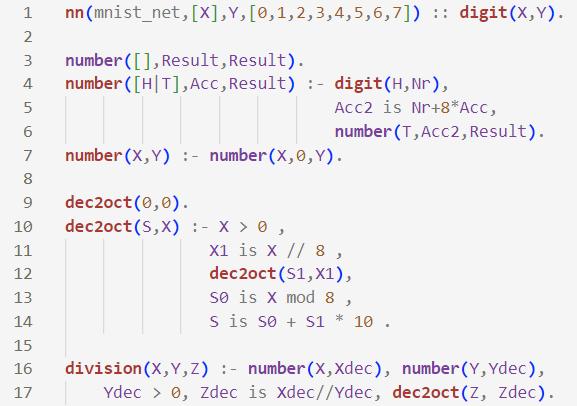
\includegraphics[scale=0.7]{problog_model.png}}
\caption{The DeepProbLog program.}
\label{fig:program}
\end{figure}

The DeepProbLog program implemented to solve the task is shown in Fig. \ref{fig:program}. The program specifies the neural annotated disjunction

\begin{equation}
    nn(mnist\_net,[X],Y,[0,1,2,3,4,5,6,7]) :: digit(X,Y).
\end{equation}

where $nn$ is a reserved functor, $mnist\_net$ is a neural network that classifies MNIST digits defining a probability distribution over the domain ${1,2,3,4,5,6,7}$ 
% composed of 8 elements since the input is an image of a base-8 digit, 
and $digit$ is the corresponding neural predicate. The output layer of the network that feeds the $digit$ neural predicate should be normalized in order to get proper probability values. In general, the neural network, apart from the output layer, could be of any kind, e.g., a recurrent network for sequence processing or a convolutional network for image processing. We decided to implement the standard convolutional network used for MNIST images since it is the more suitable neural network for MNIST images. % TODO: reference to nn

% The program contains also some rules, as shown in Fig. \ref{fig:program}. These rules permit to obtain the base-8 number from the input list of MNIST digits, convert it to a decimal number, apply the standard Prolog operator for the integer division between decimal numbers, and finally convert back the result to an octal number.

The DeepProbLog program proceeds as follows: given a training example composed of two lists of MNIST images and the result of the division in base-8, first we need to obtain the dividend and divisor from the list of images. This is done passing the images to the neural network and building the base-10 numbers from the single digits. Then the division can be calculated applying the standard Prolog operator for the integer division between decimal numbers and the result converted back to a base-8 number. The learning process can be applied based on the supervised label and on the obtained result.


% a neural predicate \texttt{digit} which maps an image of a digit $I_D$ to the corresponding natural number $N_D$.

% The ProbLog program is composed by the neural predicate \texttt{digit(x,y)} that given an image.


\subsection{Training and test sets}
Starting from the MNIST dataset we constructed the training and test sets as follows. The training set is composed of pair of images that represent single-digit base-8 numbers and the test set is composed of two lists of images that represent three-digit base-8 numbers. In both cases, the second number is a divisor of the first one. % TODO: not always 3 digits
After removing the images representing digit 8 or 9 from the MNIST training and test sets, the algorithm proceeds constructing a random number $n_1$. Then, a random divisor $n_2$ is constructed: we select a random number in the range $[1,n_1]$ and we select the nearest number that is a divisor of $n_1$. The images used to construct the two numbers are removed from the MNIST dataset. Proceeding in this way until no more pairs can be constructed, we managed to generate a training set made of $22958$ pairs and a test set made of $1462$ pairs. We fixed the random seed to obtain always the same dataset. In this way, there are no repeated images in the training and test sets but not all the MNIST images will be used: we used $45916$ of the available $48200$ training images of MNIST ($95.26\%$) and $7835$ of the available $8017$ test images of MNIST ($97.73\%$). Note that the divisors in the test set can have up to three digits, whereas the dividends are forced to have exactly three digits.
Finally, the train and test queries are generated based respectively on the train and test sets to be subsequently used by DeepProbLog during training.

\subsection{Implementation details}
In our implementation, the neural network model used to classify the MNIST digit images has a total of 44256 parameters and is a basic architecture based on the one discussed in \cite{DeepProbLog}. The model architecture can be described as follows: it consists of 2 2D-convolutional layers both with a kernel size of 5 and with respectively input channels of 1 and 6 and output channels of 6 and 16; the convolutional layers are stacked with a 2D max pooling layer, with a kernel size of 2 and stride of 2, and a rectified linear unit layer.
After these layers, the model has 3 fully connected layers of sizes 120, 84 and 8 with a rectified linear unit layer between them. The last layer is followed by a softmax layer in order to get a probability value.
The learning process optimizes the cross-entropy loss between the predicted and desired query probabilities as implemented by the function $train\_model$ that is part of the DeepProbLog framework, performing gradient accumulation instead of mini-batching.
As optimizer we used Adam with a learning rate of 0.001 for the network parameters and SGD for the logic parameters.

% \section{Results}
In this section we will present and compare the results obtained with the two approaches. 
Some results obtained from a randomly piloted battleship are considered as baseline.

For both NEAT and GP, the evolution process stores at each run the best program generated with the
relative statistical results and plots in the 'runs' folder. In this way, it is
possible to launch the program later and observe through the game interface how the battleship behaves.


\subsection{NEAT}
The NEAT algorithm managed to evolve a ANN that can reach level 42 in the game with a
fitness of 1114 after about 160 generations. The ANN is represented in Fig. \ref{fig:NEAT_best}. As we can
see the network is quite simple, with a small number of nodes and connections: it has just 10
hidden nodes and 63 enabled connections (that are represented by the solid arrows).


In Fig. \ref{fig:NEAT_fitness}, we can observe that the best fitness increases significantly in just a few particular
generations, whereas the average fitness does not grow significantly and stays under 200.
With this fitness trend, we can also notice that the speciation decreases significantly after 20
generations due to the stagnation of a lot of species: after about 60 generations, 
just the 2 elitism species will survive as shown in Fig. \ref{fig:NEAT_speciation}.

A weak point of NEAT is that the generated ANN is not really interpretable and we cannot
understand why the network produces certain output values.

\begin{figure}[ht]
\centerline{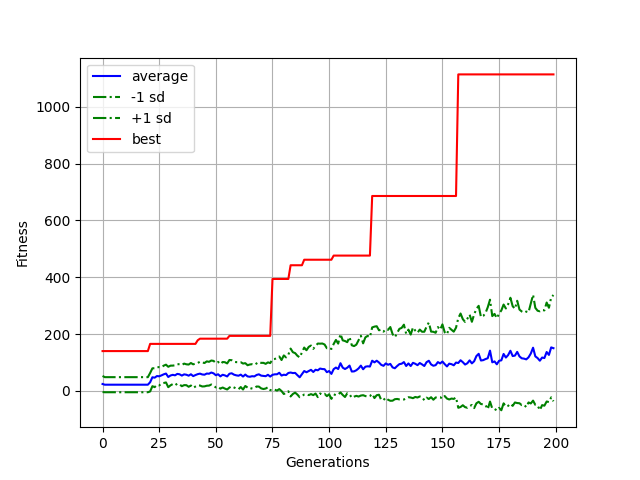
\includegraphics[scale=0.55]{NEAT_fitness.png}}
\caption{Fitness trend of the NEAT run that has generated the best ANN.}
\label{fig:NEAT_fitness}
\end{figure}


\begin{figure}[ht]
\centerline{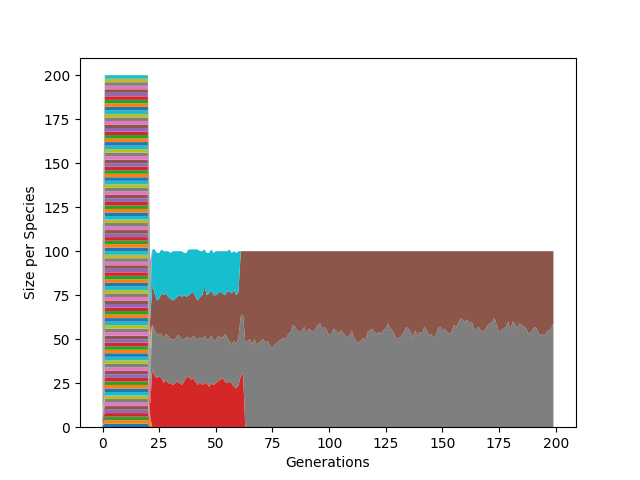
\includegraphics[scale=0.55]{NEAT_speciation.png}}
\caption{Speciation trend of the NEAT run that has generated the best ANN.}
\label{fig:NEAT_speciation}
\end{figure}


\subsection{GP}
The GP algorithm managed to evolve two tree-based programs that reach over 4000 fitness in the simulation.

The first program reaches level 151 in the
game with a fitness of 4061 during the evolution process and level 194 with a fitness of 5212
without limiting the number of frames. The tree of the program is represented in Fig. \ref{fig:GP_best1}. As
we can see the tree is quite complex, with 259 nodes and a depth of 10 (the maximum depth
allowed). In Fig. \ref{fig:GP_fitness1}, we can observe that the best fitness improves a lot in the first 60
generations reaching the frame threshold.

The second program reaches level 162 in the game with a fitness of 4342 during the evolution process and 
level 189 with a fitness of 5076 without limiting the number of frames. The tree of the program is 
represented in Fig. \ref{fig:GP_best2}. As we can see the tree is a bit less complex than the previous one, with 177 nodes 
and a depth of 10 (the maximum depth allowed). As shown in Fig. \ref{fig:GP_fitness2}, the best fitness improves significantly 
only after 100 generations, reaching the frame threshold.

In both cases, for the remaining generations, the best fitness trend increases slightly, probably also due 
to this limitation on the number of frames. The average fitness trend is smoother and follows the best trend 
with a similar increase, reaching about 3000 fitness with a large variance (over 1000).

A weak point of GP is that the generated tree is a bit complex and can be simplified a lot,
e.g. simplifying some "if\_then\_else" statements that have as condition pure boolean values as can be
seen in Fig. \ref{fig:GP_best}.

\begin{figure*}[t!]
    \centering
    \begin{subfigure}[b]{0.45\textwidth}
        \centering
        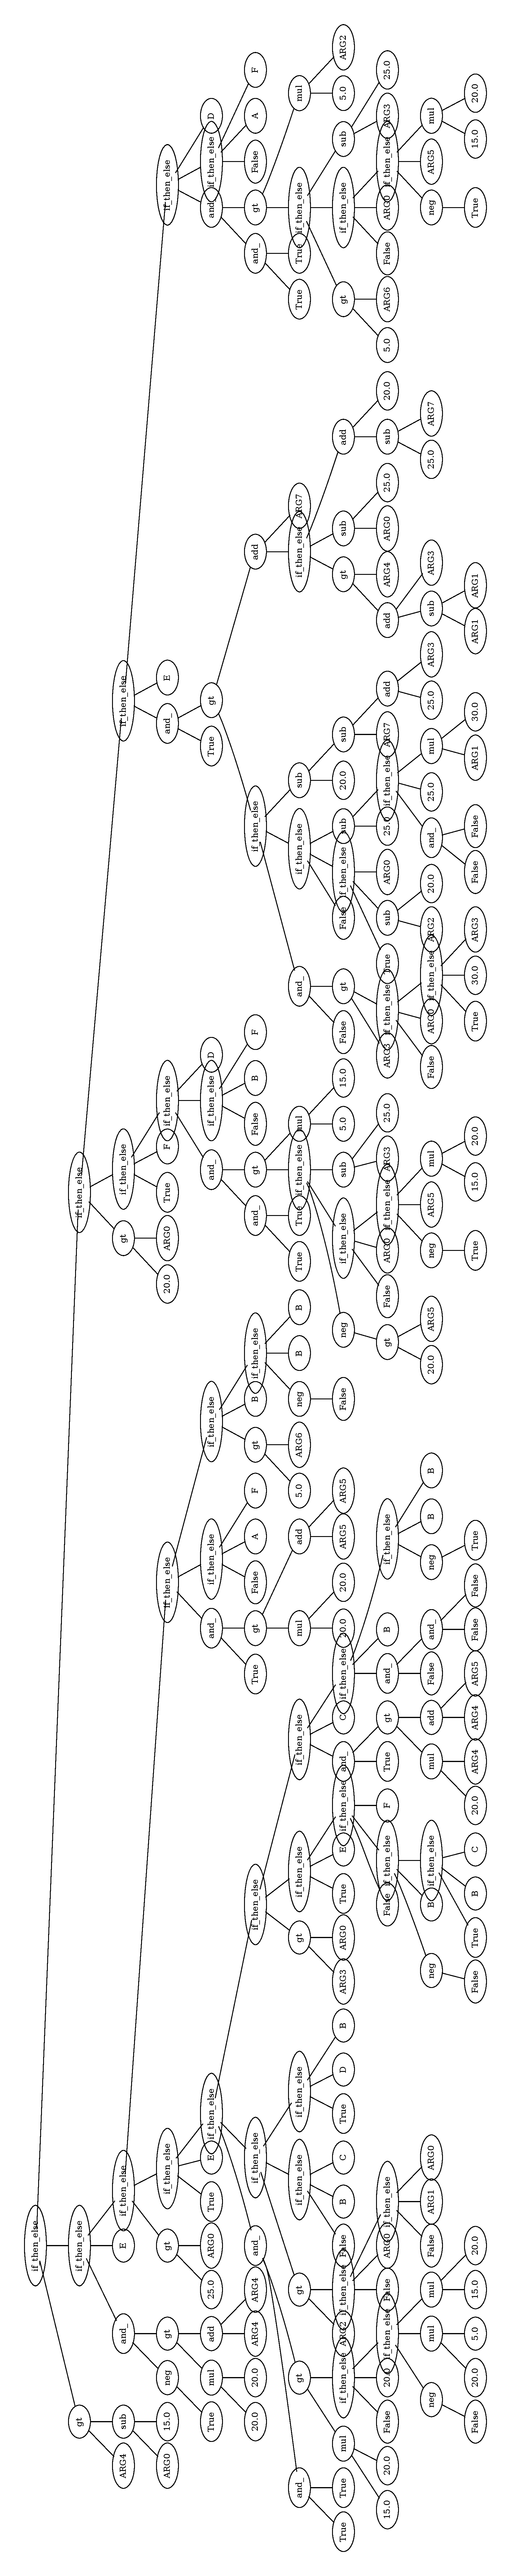
\includegraphics[scale=0.155]{GP_best1.pdf}
        \caption{}
        \label{fig:GP_best1}
    \end{subfigure}
    \hspace{1mm}
    \begin{subfigure}[b]{0.45\textwidth}
        \centering
        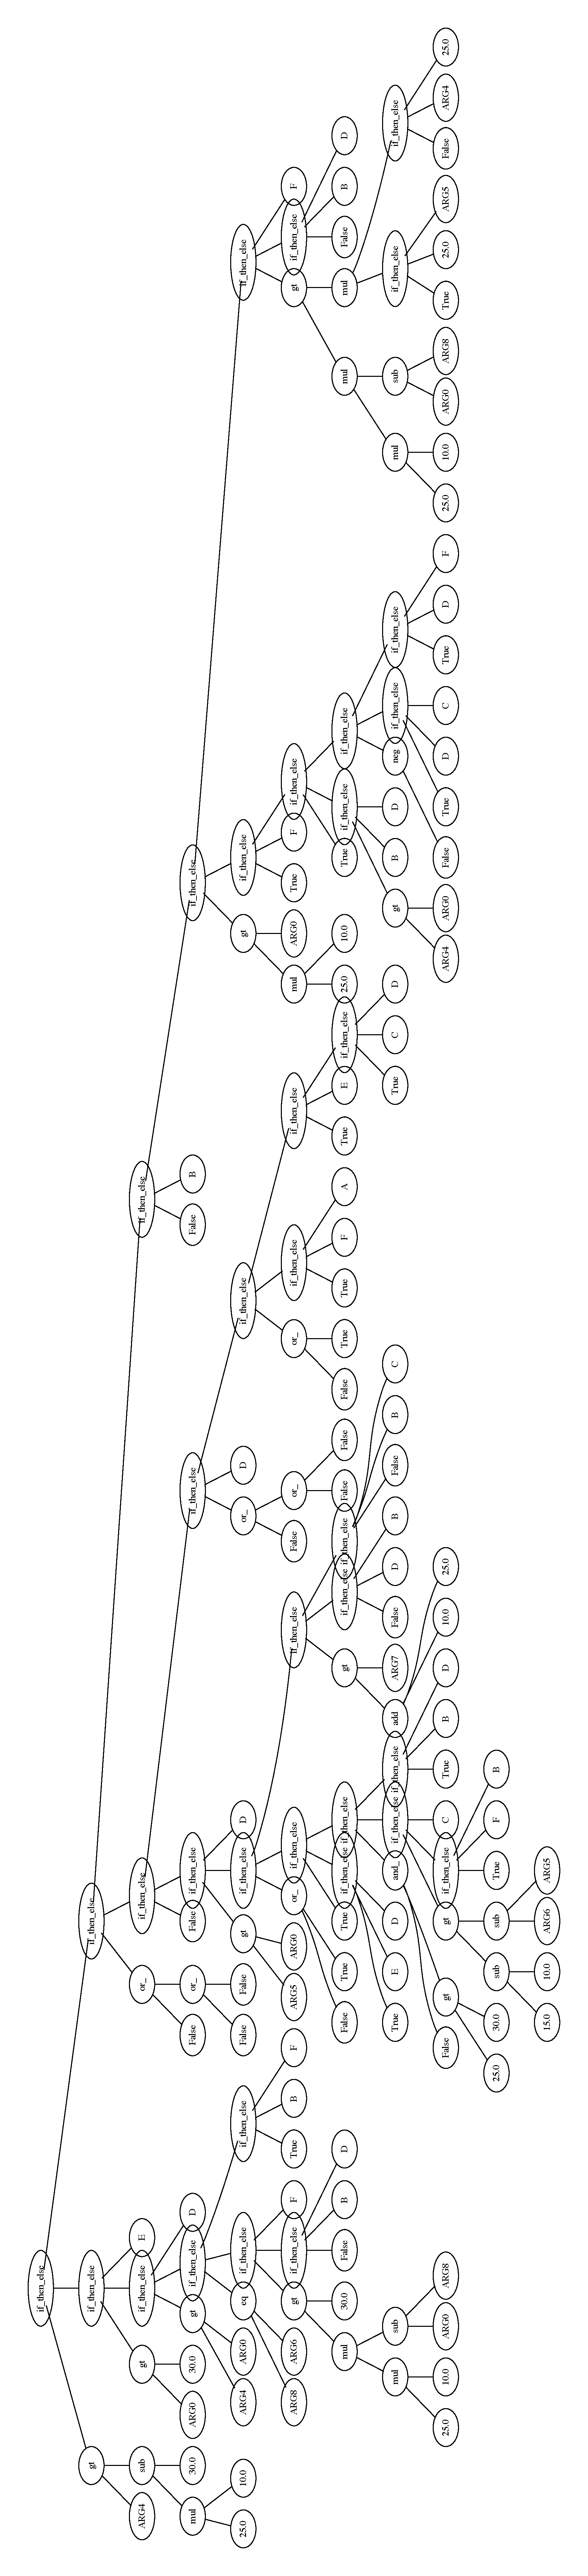
\includegraphics[scale=0.155]{GP_best2.pdf}
        \caption{}
        \label{fig:GP_best2}
    \end{subfigure}
       \caption{Best tree-based programs generated by GP.}
       \label{fig:GP_best}
\end{figure*}


\begin{figure*}[t!]
    \centering
    \begin{subfigure}[b]{0.45\textwidth}
        \centerline{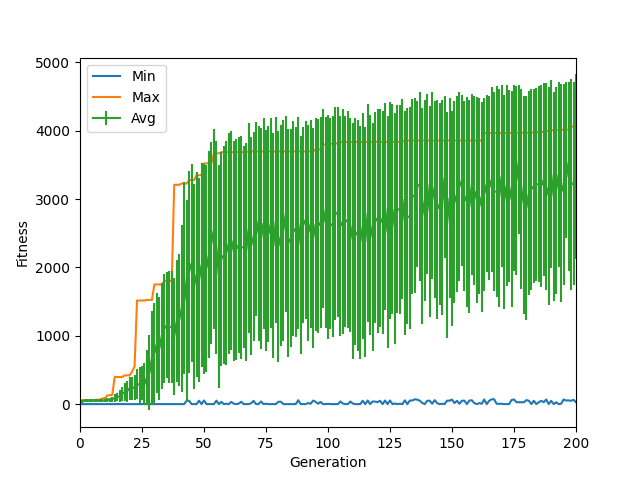
\includegraphics[scale=0.6]{GP_fitness1.png}}
        \caption{}
        \label{fig:GP_fitness1}
    \end{subfigure}
    \hfill
    \begin{subfigure}[b]{0.45\textwidth}
        \centerline{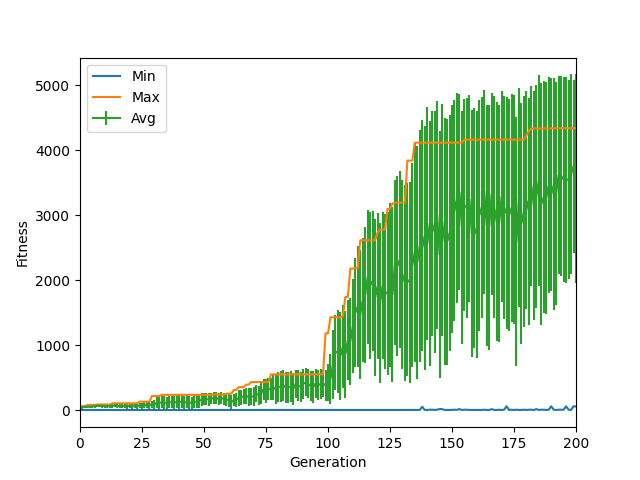
\includegraphics[scale=0.6]{GP_fitness2.png}}
        \caption{}
        \label{fig:GP_fitness2}
    \end{subfigure}
       \caption{Fitness trend of the GP runs that have generated the best programs.}
       \label{fig:GP_fitness}
\end{figure*}

\subsection{Comparison}
With both techniques, we managed to find a program that is able to play the game well,
learning to fire almost always to hit enemies while dodging their lasers.

Considering our scenario, GP demonstrated to have a bigger potential: thanks to the
tree-structure and the functions provided, it is able to learn more complex strategies
reaching level 194, much more than the best evolved ANN. NEAT, instead, struggles to
evolve the network reaching at most level 42. NEAT is probably more suitable for
tasks where a program would not be the best option or even it would be impossible
to build.

Moreover, a tree with a limited size can be more interpretable than a ANN and we can easily
provide an explanation for what the agent is doing.

Observing the agent in action we can say that both NEAT and GP agents move quite smoother, even though
neither of them resemble humans. GP agent, in the end, looks smarter and tends 
to stay in the middle of the playing area dodging all the lasers, whereas NEAT tends to
remain in the corners.

Across multiple runs, NEAT seems to obtain more stable results with respect to GP that 
manages to reach very good results only few times, as shown in Fig. \ref{fig:boxplots}. Both the techniques
find a program which performs much better than a randomly piloted battleship that on average is able 
to reach only level 3 with a fitness of about 45 as shown in Fig. \ref{fig:random_boxplot}.


\begin{figure*}
    \centering
    \begin{subfigure}[b]{0.3\textwidth}
        \centering
        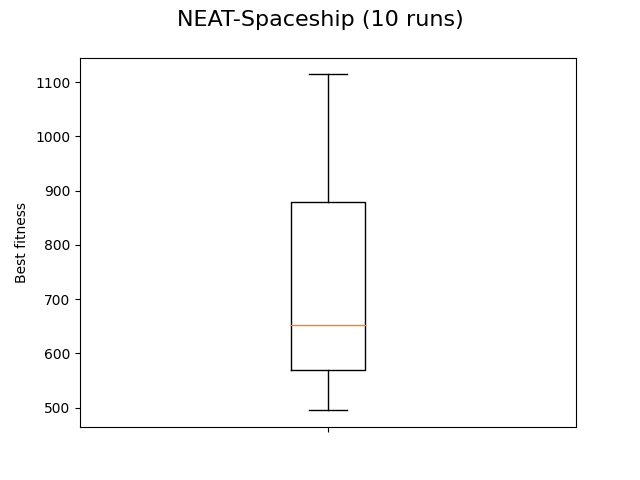
\includegraphics[scale=0.365]{NEAT_Boxplot.png}
        \caption{NEAT boxplot.}
    \end{subfigure}
    \hspace{3mm}
    \begin{subfigure}[b]{0.3\textwidth}
        \centering
        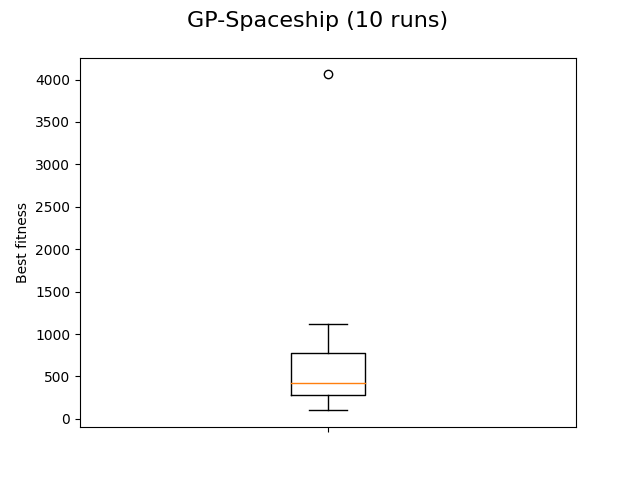
\includegraphics[scale=0.365]{GP_Boxplot.png}
        \caption{GP boxplot.}
    \end{subfigure}
    \hspace{3mm}
    \begin{subfigure}[b]{0.3\textwidth}
        \centering
        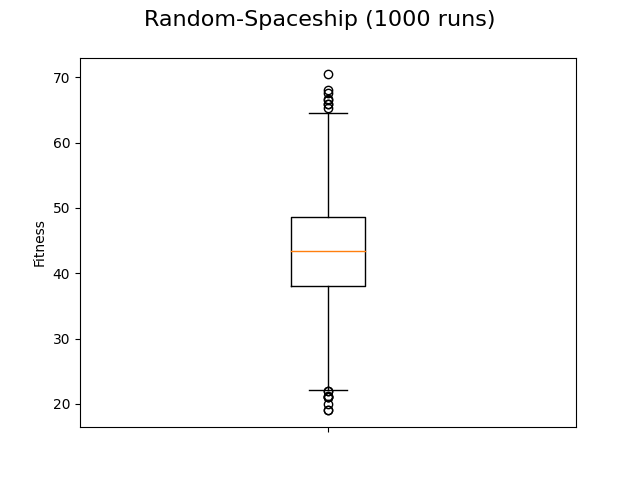
\includegraphics[scale=0.365]{Random_Boxplot.png}
        \caption{Random-piloted battleships boxplot.}
        \label{fig:random_boxplot}
    \end{subfigure}
       \caption{Comparison between the boxplots of NEAT, GP, and randomly piloted battleships.}
       \label{fig:boxplots}
\end{figure*}\

% \section{Conclusions}
\label{sec:conclusions}

As illustrated in the previous sections, DeepProbLog is a powerful framework where general-purpose neural
networks and expressive probabilistic-logical modeling and reasoning are integrated in a way that exploits the full expressiveness and strengths of both worlds. For these reasons, the framework is suitable for solving problems where both low-level data processing using deep networks and high-level reasoning using symbolic approaches are needed.

After an explanation of DeepProbLog as an extension of the ProbLog language, we have illustrated how to create and train a DeepProbLog program to solve the multi-digit MNIST octal-division task. Similarly, many more AI tasks that require both low-level perception and high-level reasoning can be efficiently solved using the DeepProbLog language.
% DeepProbLog neural probabilistic logic programming language.

% As demonstrated, NEAT and GP are very good approaches able to find a way to play the game well. Even
% though, across multiple runs, NEAT seems to obtain more stable results, GP has
% proved to have a bigger potential thanks to the tree-structured individuals and overall
% manages to reach very good results.

% One of the issues that we encountered using GP is how to manage the different input types:
% one may implement functions taking into account inputs of different types or, alternatively,
% can use a strongly typed primitive set as we have done.

% Another issue is that the execution of the algorithms takes a lot of time and
% computational resources, especially when the frame threshold is reached. Due to this, the
% number of runs and individuals should be limited.

% In the end, with this project we learned a lot about this field, in particular how it is possible to
% apply bio-inspired techniques to real-world problems and benefit from them. They have
% proved to be a valid alternative to classic back-propagation algorithms for ANN and we have learned how to
% apply them to Reinforcement Learning tasks using the fitness as a reward.



% Can use something like this to put references on a page
% by themselves when using endfloat and the captionsoff option.
\ifCLASSOPTIONcaptionsoff
  \newpage
\fi

% references section

% can use a bibliography generated by BibTeX as a .bbl file
% BibTeX documentation can be easily obtained at:
% http://mirror.ctan.org/biblio/bibtex/contrib/doc/
% The IEEEtran BibTeX style support page is at:
% http://www.michaelshell.org/tex/ieeetran/bibtex/
% \bibliographystyle{IEEEtran}
% argument is your BibTeX string definitions and bibliography database(s)
%\bibliography{IEEEabrv,../bib/paper}
%
% <OR> manually copy in the resultant .bbl file
% set second argument of \begin to the number of references
% (used to reserve space for the reference number labels box)

\printbibliography %Prints bibliography

% \begin{thebibliography}{1}

% \bibitem{Yellow-Spaceship}
% https://github.com/ph3nix-cpu/Yellow-Spaceship

% \bibitem{NEAT}
% K. O. Stanley and R. Miikkulainen, "Evolving Neural Networks through Augmenting Topologies," in Evolutionary Computation, vol. 10, no. 2, pp. 99-127, June 2002, doi: 10.1162/106365602320169811.

% \bibitem{GP}
% Koza, John R. "Hierarchical genetic algorithms operating on populations of computer programs." IJCAI. Vol. 89. 1989.

% \bibitem{NEAT-Python}
% https://neat-python.readthedocs.io/en/latest/index.html

% \bibitem{DEAP}
% https://deap.readthedocs.io/en/master/index.html

% \bibitem{PyGame}
% https://www.pygame.org/docs/

% \bibitem{repository}
% https://github.com/samuelbortolin/Bio-Inspired-Spaceship

% \end{thebibliography}

\end{document}


